\subsection{Pendahuluan}
\label{subsec:tdcrp-preliminaries}
Diberikan sebuah graf $G=(V,E)$, dengan setiap sisi $(v,w)\in E$ memiliki fungsi biaya nonnegatif $\ell(v,w)$. Karena graf merepresentasikan sebuah jaringan jalan, simpul merepresentasikan persimpangan dan sisi merepresentasikan segmen jalan pada jaringan jalan, dan fungsi biaya dihitung berdasarkan karakteristik segmen jalan (misalnya, waktu tempuh). Sebuah lintasan $P=(v_0,\ldots,v_k)$ adalah sebuah rangkaian simpul-simpul dengan $(v_i, v_{i+1}\in E)$, dan biayanya didefinisikan sebagai $\ell(P)=\sum_{i=0}^{k-1}\ell(v_i,v_{i+1})$. Tugas dari Time-Dependent Customizable Route Planning adalah menghitung  jalur terpendek dari suatu simpul asal $s$ ke simpul target $t$ dengan waktu keberangkatan dari simpul $s$ adalah $\tau_0$. Diberikan simpul asal $s$ dan simpul target $t$, penulis harus menghitung jarak $dist(s,t)$, yang didefinisikan sebagai $\ell(Opt)$ dari jalur terpendek lintasan $Opt$ pada graf $G$ dari $s$ ke $t$.

Sebuah partisi dari simpul-simpul $V$ adalah sebuah himpunan sel-sel $\mathcal{C}=\{C_0,\ldots, C_k\}, C_i\subseteq V$ dengan setiap simpul $v\in V$ terkandung didalam satu sel $C_i$. Misalkan $U$ adalah jumlah simpul dari sel terbesar. Partisi \textit{multilevel} dari $V$ adalah himpunan partisi $\{\mathcal{C}^{0},\ldots, \mathcal{C}^{L}\}$, dimana $l$ adalah \textit{level} dari partisi $\mathcal{C}^{l}$ dan $U^{l}$ merepresentasikan ukuran dari sel terbesar pada level $l$. $L$ adalah jumlah level dari  partisi \textit{multilevel}. $U^{0}=1$ atau dengan kata lain $U^{0}$ adalah $singleton$. Penulis juga menetapkan $\mathcal{C}^{L+1}=V$ untuk menandakan partisi pada level $L+1$ adalah graf orisinil. Untuk setiap level $l\leq L$ dan untuk setiap sel $C_{i}^{l}\in\mathcal{C}^l$, terdapat sebuah sel $C_{j}^{l+1}\in\mathcal{C}^{l+1} \text{ disebut sebagai \textit{supercell} dari } C_i^l$ dengan $C_i^l\subseteq C_j^{l+1}$. $c_l(v)$ adalah sel yang berisi simpul $v$ pada level $l$. Pada setiap level $l$ terdapat sisi batas dengan $endpoints$ terdapat pada sel yang berbeda pada level-$l$. Simpul batas pada level $l$ adalah simpul dengan setidaknya memiliki satu tetangga yang berada pada sel lain pada level $l$.  Untuk partisi \textit{multilevel}, simpul batas pada level $l$ juga merupakan simpul batas pada level dibawah $l$.

Dalam Time Dependent Customizable Route Planning, setiap sisi $a$ memiliki bobot berupa \textit{travel-time function} (TTF) $f_a:\Pi\rightarrow \mathbb{R}^{+}$, memetakan waktu keberangkatan ke waktu tempuh. Semua \textit{travel-time function} adalah \textit{continuous piecewiese linear function} dengan periode $\pi$ dan memiliki rentang nilai $\Pi=[0,\pi]$. Diberikan sebuah fungsi $f$, jumlah \textit{breakpoints} dari $f$ adalah $|f| $. Nilai maksimum dari $f$ didefinisikan dengan $f^{max}=\max_{\tau\in\Pi}f(\tau)$ dan nilai minimum dari $f$ didefinisikan dengan $f^{min}=\min_{\tau\in\Pi}f(\tau)$. \textit{Travel-time function} memenuhi sifat \textit{FIFO}, yaitu untuk bilangan riil positif sembarang $\sigma\leq\tau\in\Pi$, kondisi $\sigma+f(\sigma)\leq \tau+f(\tau)$ harus berlaku. Operasi \textit{link} didefinisikan dengan $link(f,g)=f+g \ \circ \ (identity+f)$, Fungsi \textit{link} juga bisa didefinisikan dengan $link(f,g)=g \star f: \tau \rightarrow g(f(\tau)+\tau) + f(\tau)$. Operasi \textit{merge} didefinisikan dengan $merge(f,g)=min(f,g):\tau \rightarrow \min \{g(\tau), f(\tau) \}$. Kedua operasi tersebut memiliki kompleksitas waktu $O(\mid f\mid +\mid g\mid )$. Diberikan rute $P=[v_1,\ldots,v_k]$, \textit{travel-time profile} (TTP) didefinisikan dengan $f_P:\Pi\rightarrow \mathbb{R}^{+}$, yang memetakan waktu keberangkatan $\tau$ (pada $v_1$) ke \textit{travel time} pada $P$ untuk menuju ke $v_k$. \textit{Arrival time function} $arr f:\tau\rightarrow f(\tau)+\tau$, memetakan waktu keberangkatan $\tau$ ke waktu kedatangan setelah melintasi sisi yang memiliki TTF $f$. 

Diberikan waktu keberangkatan $\tau$ dan simpul asal $s$ dan simpul target $t$, kueri \textit{earliest-arrival} (EA) menanyakan waktu tempuh minimum dari $s$ ke $t$ ketika berangkat pada waktu $\tau$. Kueri \textit{latest-departure} (LD) menanyakan waktu tempuh minimum yang mencapai simpul $t$ pada waktu $\tau$. Kueri profil menanyakan waktu tempuh minimum pada setiap kemungkinan waktu keberangkatan $\tau$, yaitu profil $f_{s,t}$ dari $s$ ke $t$. Kueri EA dapat ditangani dengan algoritma Time-Dependent Dijkstra yang pseudocodenya diberikan oleh algoritma~\ref{alg:td-dijkstra}. Kueri profile dapat ditangani dengan algoritma ProfileSearch yang pseudocodenya diberkan oleh algoritma~\ref{alg:profileSearch}

\subsection{Fase Prapemrosesan}
\label{subsec:tdcrp-preprocessing}
Pada tahapan prapemrosesan, penulis membuat partisi \textit{multilevel} dari graf jaringan jalan, lalu membuat topologi dari graf \textit{overlay}, dan membuat beberapa struktur data baru. Untuk membuat partisi multilevel, penulis menjalankan algoritma Inertial Flow (\cite{Schild2015}), pada graf input untuk mnghasilkan partisi level-$L$ (dengan ukuran sel maksimum $U_1,\ldots, U_{L}$ dari atas ke bawah. Pertama-tama, penulis menjalankan Inertial Flow dengan parameter $U_L$ untuk mendapatkan sel level tertinggi. Lalu, sel-sel pada lavel dibawahnya didapatkan dengan menjalankan Inertial Flow pada masing-masing sel dari level diatasnya secara paralel. Gambar~\ref{fig:mlp-inertial-flow} menunjukkan hasil dari \textit{multilevel partitioning} dengan menggunakan algoritma Inertial Flow. Setiap sel $C$ pada level 1 atau lebih tinggi diberi Id sekuensial unik di dalam superselnya. Dengan kata lain, di setiap supersel, subsel-subsel partisi dari supersel memiliki id sekuensial dari 0 hingga jumlah sel partisi dari supersel. Untuk setiap simpul $v$ penulis menyimpan Id dari sel dari simpul untuk setiap level dengan \textit{integer} 64-bit $PV(v)$, dimana bit yang lebih rendah merepresentasikan sel dari simpul di level yang lebih rendah. Hal ini bisa dicapai dengan cara: untuk setiap level dari sel simpul $v$, penulis mengalokasikan sejumlah $\lceil \log_2(\text{jumlah sel pada level } l) \rceil$-bit pada $PV(v)$ untuk menyimpan Id sel dari simpul $v$ pada level $l$. Penulis juga membuat matriks \textit{turnTables} $T_u$ untuk semua $u\in V$, dimana $T_u[i,j]$ merepresentasikan biaya untuk berbelok dari sisi masuk ke-$i$ dan sisi keluar ke-$j$ dari simpul $u$. Biaya untuk berbelok dari sisi masuk ke-$i$ dan sisi keluar ke-$j$ dari simpul $u$ bisa ditentukan oleh pengguna dan biasanya biaya ditentukan berdasarkan tipe belokan (contoh, \textit{u turn},  \textit{right turn}, \textit{left turn}). Untuk setiap sisi keluar $(v,w)$, penulis menyimpan \textit{head order} titik \textit{entry}(posisi dari sisi relatif terhadap sisi masuk $w$) dan \textit{head point} (simpul $w$). Untuk setiap sisi masuk $(v,w)$, penulis menyimpan \textit{tail order}/titik \textit{exit}(posisi dari sisi relatif terhadap sisi keluar $v$) dan \textit{tail point} (simpul $v$). Lihat gambar~\ref{fig:crp-exit-entry-point} untuk ilustrasi mengenai titik \textit{entry}/\textit{exit}.

\begin{figure}[h]
    \centering

    \begin{subfigure}[b]{0.45\textwidth}
        \centering
        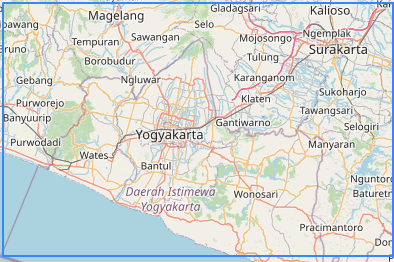
\includegraphics[width=\linewidth]{figures/original_road_networks.png}
        \caption{Graf jaringan jalan untuk peta Openstreetmap wilayah Surakarta, Daerah Istimewa Yogyakarta, dan Klaten}
        \label{fig:a}
    \end{subfigure}
    \hfill
    \begin{subfigure}[b]{0.45\textwidth}
        \centering
        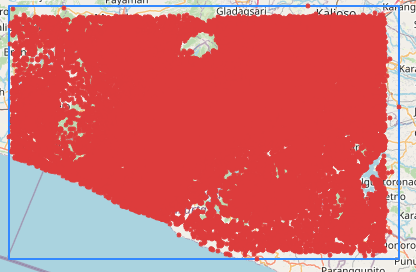
\includegraphics[width=\linewidth]{figures/partition_level_5.png}
        \caption{Partisi level 5 dengan ukuran $U_5=2^{20}$}
        \label{fig:b}
    \end{subfigure}

    \begin{subfigure}[b]{0.45\textwidth}
        \centering
        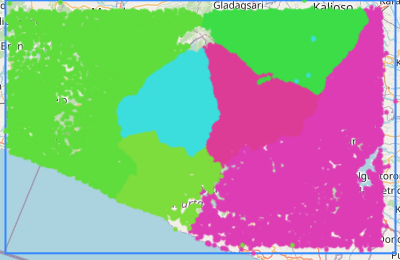
\includegraphics[width=\linewidth]{figures/partition_level_4.png}
        \caption{Partisi level 4 dengan ukuran $U_4=2^{17}$}
        \label{fig:c}
    \end{subfigure}
    \hfill
    \begin{subfigure}[b]{0.45\textwidth}
        \centering
        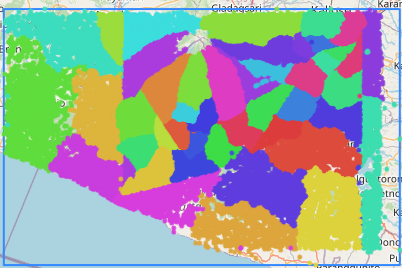
\includegraphics[width=\linewidth]{figures/partition_level_3.png}
        \caption{Partisi level 3 dengan ukuran $U_3=2^{14}$}
        \label{fig:d}
    \end{subfigure}

   
    \begin{subfigure}[b]{0.45\textwidth}
        \centering
        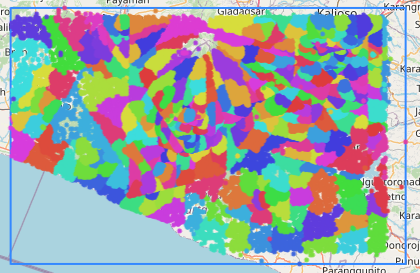
\includegraphics[width=\linewidth]{figures/partition_level_2.png}
        \caption{Partisi level 2 dengan ukuran $U_w=2^{11}$}
        \label{fig:c}
    \end{subfigure}
    \hfill
    \begin{subfigure}[b]{0.45\textwidth}
        \centering
        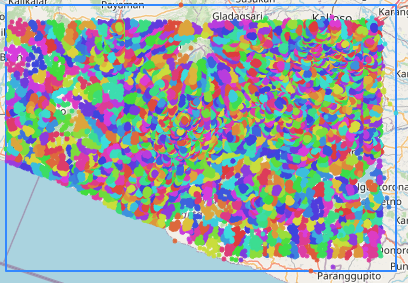
\includegraphics[width=\linewidth]{figures/partition_level_1.png}
        \caption{Partisi level 1 dengan ukuran $U_1=2^{8}$}
        \label{fig:d}
    \end{subfigure}

    \caption{Partisi \textit{multilevel} untuk graf jaringan jalan peta Openstreetmap wilayah Surakarta, Daerah Istimewa Yogyakarta, dan Klaten. Graf memiliki jumlah simpul sebanyak 481.978 dan jumlah sisi sebanyak 1.222.793.}
    \label{fig:mlp-inertial-flow}
\end{figure}

\begin{figure}[H]
    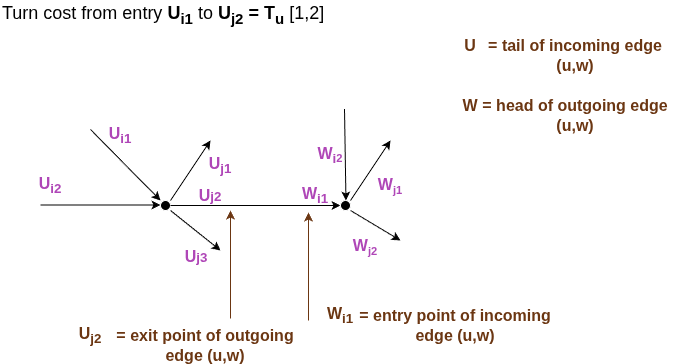
\includegraphics[scale=0.4]{figures/turn_cost_exit_entry.png}
    \caption{titik \textit{exit}, titik \textit{entry}, \textit{head point}, dan \textit{tail point} dari sisi $(u,w)$}
    \label{fig:crp-exit-entry-point}
\end{figure}


Untuk setiap sisi batas $(u,v)$, penulis menyimpan simpul \textit{overlay} $u'_{H}$ dan $v_{H}''$, dimana simpul $u'_{H}$  adalah simpul \textit{exit} dari sel $c_1(u)$ dan $v_{H}''$ adalah simpul \textit{entry} dari sel $c_1(v)$. Jika sisi $(v,u)$ juga terdapat dalam graf, maka kita juga menambahkan simpul $v'_H$ dan $u''_{H}$. Untuk meningkatkan lokalitas, penulis mengurutkan Id dari simpul \textit{overlay} sedemikian hingga simpul batas dengan level tertinggi memiliki Id terendah, diikuti dengan simpul batas dengan level tetinggi kedua, dan seterusnya. Gambar~\ref{fig:crp-overlay2} menunjukkan ilustrasi dari sisi batas dan simpul \textit{overlay}/batas. Penulis membangun struktur data berupa hash table dengan key yang merupakan sebuah struct berisi beberapa field, yaitu: Id dari simpul, \textit{exit/entry order} dari sisi batas milik simpul, tipe simpul (\textit{exit}/\textit{entry}) dengan value nya adalah Id dari simpul \textit{overlay}. Untuk menyimpan bobot dari sisi-sisi jalan pintas yang menghubungkan simpul-simpul \textit{overlay}/batas pada setiap sel di setiap level, penulis membuat struktur data \textit{array} satu dimensi bobot sisi jalan pintas W. Untuk setiap sel $C$  di dalam graf \textit{overlay} di setiap level, penulis menyimpan $p_C$ (jumlah dari titik \textit{entry} dari sel), $q_C$ (jumlah dari titik \textit{exit} dari sel), dan $f_C$ (posisi di dalam \textit{array} $W$, dimana entri pertama dari matrix bobot dari sel $C$ disimpan), kita dapat mendapatkan bobot/biaya dari sisi jalan pintas antara titik \textit{entry} ke-$i$ dan titik \textit{exit} ke-$j$ dari sel $C$ dari $W[f_C+i\cdot q_C + j]$. Untuk dapat memetakan posisi simpul diantara simpul-simpul \textit{exit} atau \textit{entry} dari sel simpul ke Id dari simpul overlay nya, penulis membuat \textit{hash table} yang memetakan posisi \textit{entry}/\textit{exit} ke-$i$ dari sel $C$ pada level $l$ ke Id dari simpul \textit{overlay} yang bersesuaian. Untuk setiap simpul \textit{overlay} $v$, penulis juga menyimpan \textit{array} berukuran $L$ yang setiap indeksnya menyimpan posisi titik \textit{entry/exit} dari simpul pada sel pada level indeks dimana simpul berada.



\begin{figure}[H]
    \centering
    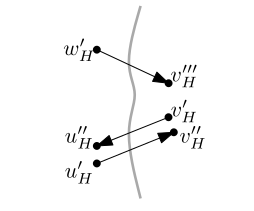
\includegraphics[]{figures/overlay_crp.png}
    \caption{graf \textit{overlay} yang terdiri dari sisi batas $(u,v)$, $(v,u)$, dan $(w,v)$ menghasilkan simpul \textit{overlay} $u'_{H},v_H'',v'_H,u''_H,w'_H, \text{ dan }v'''_H$ }
    \label{fig:crp-overlay2}
\end{figure}




\subsection{Fase Kustomisasi Tidak Bergantung Pada Waktu}
\label{subsec:tdcrp-kustomisasi}
Pada fase kustomisasi, penulis membuat sisi-sisi jalan pintas yang menghubungkan antara simpul \textit{entry} dan simpul \textit{exit} dari setiap sel dengan menggunakan bobot sisi yang terbaru. Penulis juga membangun \textit{array} bobot sisi-sisi jalan pintas W. Untuk membuat sisi-sisi jalan pintas, penulis menjalanakan algoritma Dijkstra secara \textit{bottom-up}. Untuk setiap sel $C$ dari graf \textit{overlay} level 1, penulis menjalankan algoritma \textit{turn-aware} Dijkstra pada setiap simpul \textit{entry} dari sel $C$ ke semua simpul \textit{exit} dari sel $C$. Untuk setiap sel $C$ dari graf level i (untuk i > 1), penulis menjalankan algoritma \textit{turn-aware} Dijkstra pada setiap simpul \textit{entry} ke semua simpul \textit{exit} dari sel $C$. Untuk level i > 1, algoritma Dijkstra dijalankan pada subgraf dari $H_{i-1}$ menggunakan sisi-sisi jalan pintas dari subsel-subsel dari sel $C$ yang mana cenderung lebih cepat jika dibandingkan dengan kustomisasi pada level 1. Untuk mengakselerasi fase kustomisasi, penulis menjalankan kustomisasi dari setiap sel secara \textit{multithreaded} dan menjalankan algoritma Dijkstra dari setiap simpul \textit{entry} secara \textit{multithreaded}. Gambar~\ref{fig:clique-crp} menunjukkan ilustrasi dari hasil kustomisasi. Pesudocode untuk algoritma kustomisasi pada level 1 ditunjukkan pada Algoritma~\ref{alg:crp-customization-level1} dan Algoritma~\ref{alg:crp-customization-levelhigher} untuk level $l>1$. Misalkan $K$ adalah jumlah partisi pada graf \textit{overlay} level 1 dan diasumsikan setiap partisi memiliki jumlah simpul yang sama ($|C_1|=|C_2|=\ldots =|C_K|$), maka kompleksitas dari algoritma kustomisasi adalaah $O(|E|+|V|\log \frac{|V|}{K})$.

\begin{figure}[H]
    \centering
    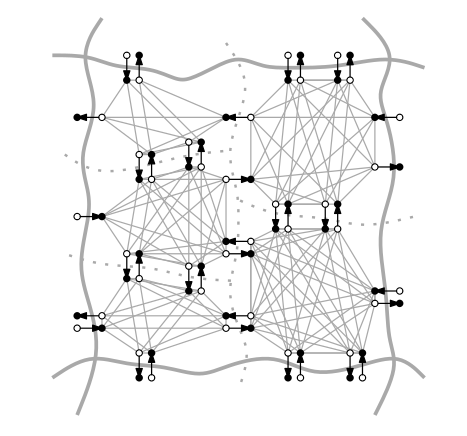
\includegraphics[]{figures/clique.png}
    \caption{graf overlay hasil kustomisasi}
    \label{fig:clique-crp}
\end{figure}




\begin{algorithm}
\caption{BUILDOVERLAYLEVELONE membuat \textit{clique} pada setiap sel-sel level 1 dan membuat \textit{array} bobot \textit{shortcut arcs} $W$}
\label{alg:crp-customization-level1}
\resizebox{\textwidth}{!}{%
\begin{minipage}{\textwidth}
\scriptsize
\begin{algorithmic}[1]
\setstretch{0.9}
\Procedure{BUILDOVERLAYLEVELONE}{$G, OG$}
    \For {$(cellId, cell) \in OG.CellsInLevel[1]$} \Comment{buat \textit{clique} dan \textit{array} bobot \textit{shortcut arcs} $W$  pada setiap sel level 1 }
        \For {$i = 0 \textbf{ to } cell.numEntryPoints$}
            \State $enVertex \gets OG.entryPoint[cell, i]$  \Comment{Dijkstra dari $entryVertex$ ke semua $exitVertex$ dari sel $cellId$}
            \State $enVertexEntryPos \gets G.entryPos[enVertex.originalEdge, enVertex]$
            \State $info \gets \emptyset$
            \State $oInfo \gets \emptyset$
            \State $Q \gets \emptyset: PriorityQueue$
            \State $info[enVertexEntryPos] \gets 0$
            \State $Q.insert(0, (enVertex, enVertexEntryPos))$
            \While{$Q \neq \emptyset$}
                \State $((u, uEntryPos), uTT) \gets Q.extractMin()$
                \For {$(v, oArc,exitPoint, turn) \in  G.E[u, uEntryPos]$}
                    \State $v \gets oArc.head$
                    \State $newTT \gets uTT + turn.cost + oArc.weight$
                    \State $vCellId \gets G.cellId[v]$
                    \If {$vCellId = cellId$}
                        \State $vEntryPos \gets oArc.entryPos$ \Comment{$v$ masih satu sel dengan $cellId$}
                        \State $((\cdot),vVisited) \gets info[vEntryPos]$
                        \If{$vVisited = false \textbf{ or } newTT < info[vEntryPos]$}
                            \State $info[vEntryPos] \gets newTT$
                            \State $Q.InsertOrDecreaseKey(newTT, (v, vEntryPos))$
                        \EndIf 
                    \Else 
                        \State $exitOverlay \gets G.overlayVertex[u, exitPoint, true]$ \Comment{$v$ tidak satu sel dengan $cellId$ }
                        \State $exitOverlayVisited \gets oInfo[exitOverlay]$  \Comment{$u$ adalah $exitVertex$ dari $cellId$}
                        \If {$exitOverlayVisited = false \textbf{ or } uTT + turn.cost < oInfo[exitOverlay]$}
                            \State $oInfo[exitOverlay] \gets uTT + turn.cost $
                        \EndIf 
                    \EndIf 
                \EndFor 
            \EndWhile 

            \For {$j =0  \textbf{ to }  cell.numExitPoints$}
                \State $exitVertex \gets OG.exitPoint[cell, j]$ \Comment{simpan bobot dari sisi \textit{shortcut} $(enVertex, exitVertex)$}
                \State $((\cdot), exitPointVisited) \gets oInfo[exitVertex]$
                \If{$exitPointVisited = false$}
                    \State $OG.W[cell.cellOffset + i \cdot cell.numberExitPoints + j]  \gets \infty$
                \Else 
                    \State $OG.W[cell.cellOffset + i \cdot cell.numberExitPoints + j]  \gets oInfo[exitPoint]$
                \EndIf 
            \EndFor 
        \EndFor
    \EndFor 
\EndProcedure
\end{algorithmic}
\end{minipage}%
}
\end{algorithm}

\begin{algorithm}
\caption{BUILDOVERLAY membuat \textit{clique} pada setiap sel-sel level $l>1$ dan membuat \textit{array} bobot \textit{shortcut arcs} $W$}
\label{alg:crp-customization-levelhigher}
\resizebox{\textwidth}{!}{%
\begin{minipage}{\textwidth}
\scriptsize
\begin{algorithmic}[1]
\setstretch{0.9}
\Procedure{BUILDOVERLAY}{$G, OG, l$}
    \For {$(cellId, cell) \in OG.CellsInLevel[l]$} \Comment{buat \textit{clique} dan \textit{array} bobot \textit{shortcut arcs} $W$  pada setiap sel level $l$ }
        \For {$i = 0 \textbf{ to } cell.numEntryPoints$}
            \State $enVertex \gets OG.entryPoint[cell, i]$  \Comment{Dijkstra dari $entryVertex$ ke semua $exitVertex$ dari sel $cellId$}
            \State $info \gets \emptyset$
            \State $oInfo \gets \emptyset$
            \State $Q \gets \emptyset: PriorityQueue$
            \State $info[enVertex] \gets 0$
            \State $Q.insert(0, (enVertex))$
            \While{$Q \neq \emptyset$}
                \State $((u), uTT) \gets Q.extractMin()$
                \For {$(exitVertex, wOffset) \in  OG.E[u, l-1]$} \Comment{\textit{traverse} semua sisi \textit{shortcut} $(enVertex,exitVertex)$ pada level $l-1$ }
                    \State $shortcutWeight \gets OG.W[wOffset]$
                    \State $newTT \gets uTT + shortcutWeight$
                    \State $(oldExitTT, exitVisited) \gets info[exitVertex]$
                    \If{$exitVisited = false \textbf{ or } newTT < oldExitTT$}
                        \State $info[exitVertex] \gets newTT$
                        \State $exitNeighborVertex \gets exitVertex.neighbor$ \Comment{\textit{traverse} neighbor dari $exitVertex$ yang berbeda sel dengan $sel$ dari $exitVertex$ pada level $l-1$}
                        \If {$TRUNCATEDTOEVEL(exitNeighborVertex.cellId, l) = cellId$}
                            \State $boundaryArcWeight \gets  exitVertex.edge.weight$ \Comment{$exitNeighborVertex$ masih satu sel dengan $exitVertex$ pada level $l$}
                            \State $newNeighborTT \ \gets newTT + boundaryArcWeight $
                            \State $(oldNTT, neighborVisited) \gets info[exitNeighborVertex]$
                            \If {$neighborVisited=false \textbf{ or } newNeighborTT < oldNTT$} 
                                \State $info[exitNeighborVertex] \gets newTT +boundaryArcWeight $
                                \State $Q.InsertOrDecreaseKey(info[exitNeighborVertex], exitNeighborVertex)$
                            \EndIf 
                        \EndIf 
                    \EndIf
                \EndFor 
            \EndWhile 

            \For {$j =0  \textbf{ to }  cell.numExitPoints$}
                \State $exitVertex \gets OG.exitPoint[cell, j]$ \Comment{simpan bobot dari sisi \textit{shortcut} $(enVertex, exitVertex)$}
                \State $((\cdot), exitPointVisited) \gets oInfo[exitVertex]$
                \If{$exitPointVisited = false$}
                    \State $OG.W[cell.cellOffset + i \cdot cell.numberExitPoints + j]  \gets \infty$
                \Else 
                    \State $OG.W[cell.cellOffset + i \cdot cell.numberExitPoints + j]  \gets oInfo[exitPoint]$
                \EndIf 
            \EndFor 
        \EndFor
    \EndFor 
\EndProcedure
\end{algorithmic}
\end{minipage}%
}
\end{algorithm}


\subsection{Fase Kueri Tidak Bergantung Pada Waktu}
\label{subsec:tdcrp-kueri}
Kueri pada Customizable Route Planning dilakukan dengan algoritma Turn Aware Multilevel Bidirectional Dijkstra (TA-MLBD). Kueri dari $s$ ke $t$ terdiri dari tiga bagian: prefiks maksimal di $c(s)$, suffiks maksimal $c(t)$, dan graf overlay $H$ yang berada diantara keduanya. Karena jarak antara simpul-simpul \textit{overlay}/batas pada graf overlay $H$ dan graf $G$ memiliki jarak yang sama, maka rute terpendeknya akan sama dengan rute terpendek pada graf $G$ (\cite{Delling2015}). Input dari kueri adalah sisi asal $a_s$, sisi target $a_t$, graf $G$, dan graf \textit{overlay} $H =\cup_i H_i$. Tugas dari kueri adalah menghitung rute terpendek antara simpul \textit{head} $s$ dari $a_s$ dan simpul \textit{tail} dari $a_t$. Algoritma ini menggunakan empat \textit{priority queue}, yaitu \textit{forward overlay priority queue}(forwardOverlayPQ), \textit{backward overlay priority queue}(backwardOverlayPQ), \textit{forward original priority queue}(forwardPQ), dan \textit{backward original priority queue}(backwardPQ). \textit{Key} dari \textit{original priority queue}(PQ) TA-MLD adalah $(v,i,d)$, dimana $v$ adalah simpul $i$ adalah posisi titik \textit{entry} pada $v$, dan $d$ adalah label waktu tempuh. Algoritma menginisialisasi $(s,i,d)$ dengan $(s,i,0)$ dan $(t,i,d)$ dengan $(t,i,0)$. Dengan representasi seperti ini, ketika kita sedang melakukan relaksasi sisi $(u,v)\in E$, posisi titik \textit{entry} dari $u$ adalah $i$ dan posisi titik \textit{exit} dari sisi $(u,v)$ adalah $j$, penulis dapat mendapatkan biaya \textit{turn}  dari sisi masuk ke-$i$ dan sisi keluar ke-$j$ dari simpul $u$  dari matriks \textit{turnTables}.

Diberikan simpul $v\in V$, \textit{query level} $l_{st}(v)$ adalah level tertinggi sedemikian hingga sel dari $v$ tidak sama dengan sel dari $s$ atau $t$. $l_{st}(v)$ adalah level $i$ tertinggi sedemikian hingga $c_i(v)\cap\{s,t\}=\emptyset$. $l_{st}(v)$ dihitung dengan $l_{st}(v)=\min\{MSD(PV(s), PV(v)), MSD(PV(t), PV(v))\}$, dimana $MSD(PV(s), PV(v))=\text{level tertingi dimana bit dari } PV(s) \text{ dan }PV(v) \text{ berbeda}$. \textit{Overlay priority queue} memilki key $(v, l_{st}(v)),\text{ dimana } v\in V$.

Algoritma $TAMLBD$ menyimpan waktu terpendek tentatif $\mu$ yang nilainya diinisialisasi dengan $\infty$. Algoritma \textit{forward search} dimulai dengan mengeksplorasi simpul-simpul yang berada pada sel yang sama dengan simpul $s$ pada level 1, sedangkan \textit{backward search} dimulai dengan mengeksplorasi simpul-simpul yang berada pada sel yang sama dengan simpul $t$ pada level 1. Algoritma mulai mengeksplorasi simpul-simpul tetangga dari simpul $v$ yang berbeda dari sel $s$ atau $t$ pada level 1 ketika \textit{query level} $l_{st}(v)>0$, pada tahap ini algoritma menjalankan algoritma Dijkstra pada graf \textit{overlay} pada level $l_{st}(v)$ memanfaatkan sisi-sisi \textit{shortcuts} yang sudah dibuat pada fase kustomisasi. Pada saat melakukan relaksasi sisi, algoritma melakukan pengecekan apakah simpul $v$ (yang merupakan $head$ dari sisi $(u,v)$ yang sedang direlaksasi) apakah sudah di kunjungi pada kedua pencarian. Jika simpul $v$ telah dikunjungi oleh \textit{forward search} dan \textit{backward search}, maka nilai waktu tempuh terpendek tentatif $\mu$ diperbarui. Apabila simpul $v$ (yang merupakan $head$ dari sisi $(u,v)$ yang sedang direlaksasi) memiliki $l_{st}(v) = 0$, maka ketika simpul $v$ berada dalam keadaan \textit{settled}, algoritma akan mengeksplorasi simpul-simpul tetangga dari $v$ yang berada pada sel yang sama dengan sel simpul $s$ atau $t$ pada level 1.

Penulis melakukan beberapa optimasi untuk mempercepat algoritma kueri. Pada saat relaksasi sisi jalan pintas $(u,v)$ atau $(v,u)$ pada subrutin Bidirectional Overlay Graph Dijkstra, subrutin menyimpan waktu tempuh terpendek dari simpul $v$ dan tidak langsung menambahkan/memperbarui simpul \textit{exit} $v$ ke $forwardOverlayPQ$ atau $backwardOverlayPQ$, subrutin langsung melakukan relaksasi sisi batas $(v,w)\in E$. Hal ini mengurangi jumlah operasi Priority Queue secara signifikan. Penulis juga melakukan optimisasi dengan cara mengalokasikan ukuran awal setiap struktur data yang dibutuhkan kueri dengan $\max\{len(c_1(s)),len(c_1(t))\}$, dimana $len(c_1(v))$ adalah jumlah simpul yang terletak pada sel yang mengandung simpul $v$. Implementasi Priority Queue dari algoritma kueri menggunakan varian Rank Pairing-Heap Priority Queue (\cite{Haeupler2009}) karena operasi \textit{decreaseKey} dari varian ini memiliki kompleksitas waktu terarmortisasi $O(1)$ dan operasi \textit{insert} memiliki kompleksitas waktu $O(1)$ akan membuat waktu eksekusi algoritma kueri semakin cepat. Algoritma~\ref{alg:crp-tamlbd} menunjukkan \textit{pseudocode} dari algoritma kueri Customizable Route Planning.


\begin{algorithm}
\caption{TAMLBD}
\label{alg:crp-tamlbd}
\resizebox{\textwidth}{!}{%
\begin{minipage}{\textwidth}
\scriptsize
\begin{algorithmic}[1]
\setstretch{0.9}
\Procedure{TAMLBD}{$as, at, G, OG$}
    \State $s \gets as.head$
    \State $t \gets at.tail$
    \State $sEntryPos \gets G.entryPos[as,s]$
    \State $tEntryPos \gets G.entryPos[at,t]$
    \State $fInfo, bInfo \gets \emptyset$
    \State $fQ,bQ \gets  \emptyset: PriorityQueue$
    \State $foQ,boQ \gets  \emptyset: PriorityQueue$
    \State $shortest \gets \infty$
    \State $fQ.insert(s, sEntryPos)$
    \State $bQ.insert(t, tEntryPos)$
    \While{$|fQ|+|foQ| > 0 \textbf{ dan } |bQ|+|boQ| > 0$ }
        \If {$\min\{\min_{fQ}, \min_{foQ} \} +\min\{\min_{bQ}, \min_{boQ} \} > shortest $}
            \State \textbf{break}
        \EndIf 
        \State $minQ=\min \{ \min_{fQ}, \min_{bQ}  \}$
        \State $minOQ=\min \{ \min_{foQ}, \min_{boQ}  \}$
        \If {$minQ < minOQ$}
            \State \Call{BDTurnAwareDijkstra}{$s,t,fInfo,bInfo,fQ, bQ, foQ, boQ, G, OG, shortest$}
        \Else 
             \State \Call{BDTurnAwareOverlayDijkstra}{$s,t,fInfo,bInfo,fQ, bQ, foQ, boQ, G, OG, shortest$}
        \EndIf
    \EndWhile   
    \State \textbf{return} $shortest, $ \Call{PATHUNPACKING}{$G,OG,fInfo,bInfo,PV(s),PV(t)$}
\EndProcedure
\end{algorithmic}
\end{minipage}%
}
\end{algorithm}


\begin{algorithm}
\caption{BidirectionalTurnAwareDijkstra}
\resizebox{\textwidth}{!}{%
\begin{minipage}{\textwidth}
\scriptsize
\begin{algorithmic}[1]
\setstretch{0.9}
\Procedure{BDTurnAwareDijkstra}{$s,t,fInfo,bInfo,fQ, bQ, foQ, boQ, G, OG, shortest$}
    \State $minRankF \gets fQ.findMin()$
    \State $minRankB \gets bQ.findMin()$
    \If {$minRankF <  minRankB$}
       \State  $((u, uEntryPos), \cdot) \gets fQ.deleteMin()$ \Comment{\textit{forward search} pada graf $G$}
        \For{$(oArc, turn, v) \in G.E[u,uEntryPos]$}
            \State $l_{st}(v) \gets \min\{MSD(PV(s), PV(v)), MSD(PV(t), PV(v))\}$
            \If{$l_{st}(v)=0$}
                \State $newTT \gets fInfo[uEntryPos].tt + oArc.weight + turn.cost$
                \State \Call{RELAX}{$v,u,uEntryPos, oArc, false, newTT,fInfo,bInfo, fQ,bQ, G, shortest$}
            \Else 
                \State \Call{RELAXOVERLAY}{$v,u,uEntryExitPos,oArc,false, shortest, G, newTT, l_{st}(v), fInfo, bInfo, foQ, boQ$}
            \EndIf 
        \EndFor 
    \Else 
        \State $((u, uExitPos), \cdot) \gets bQ.deleteMin()$ \Comment{\textit{backward search} pada graf $G$}
        \For{$(iArc, turn, v) \in  G.\overleftarrow{E}[u,uExitPos]$}
            \State $l_{st}(v) \gets \min\{MSD(PV(s), PV(v)), MSD(PV(t), PV(v))\}$
            \If{$l_{st}(v)=0$}
                \State $newTT\gets bInfo[uExitPos].tt + iArc.cost +turn.cost$
                \State \Call{RELAX}{$v,u,uExitPos,iArc,true,newTT,fInfo,bInfo,fQ,bQ, G, shortest$}
            \Else
                \State \Call{RELAXOVERLAY}{$v,u,uEntryExitPos,iArc, true, shortest, G, newTT, l_{st}(v), fInfo,bInfo, foQ,boQ$}
            \EndIf
        \EndFor 
        
    \EndIf 
\EndProcedure
\end{algorithmic}
\end{minipage}%
}
\end{algorithm}


\begin{algorithm}
\caption{RELAX}
\resizebox{\textwidth}{!}{%
\begin{minipage}{\textwidth}
\scriptsize
\begin{algorithmic}[1]
\setstretch{0.9}
\Procedure{RELAX}{$v,u,uEntryPos, Arc, backward, newTT, fInfo,bInfo, fQ,bQ, G, shortest$}
    \If {$backward = false$}
        \State $vEntryPos \gets G.entryPos[arc,v] $
        \State $((\cdot), vVisited) \gets fInfo[vEntryPos]$
        \If {$newTT < fInfo[vEntryPos].tt \textbf{ or } vVisited = false$}
            \State $fInfo[vEntryPos] \gets (newTT, u , uEntryExitPos)$ \Comment{relaksasi sisi keluar $(u,v)\in G.E$}
            \State $fQ.InsertOrDecreaseKey(newTT, (v, vEntryPos))$ 
            \For{$(voArc, vExitPos, turn, \cdot) \in G.E[v, arc.entryPos]$} 
                \State $((\cdot), visitedByBackward) \gets bInfo[vExitPos]$ \Comment{cek apakah $v$ sudah dikunjungi pada kedua \textit{search}}
                \If{$visitedByBackward = true$}
                    \State $newTT \gets fInfo[vEntryPos].tt + turn.cost + binfo[vExitPos].tt$
                    \If{$newTT < shortest$}
                        \State $shortest=  newTT$
                    \EndIf
                \EndIf 
            \EndFor 
        \EndIf 
    \Else 
        \State $vExitPos \gets G.exitPos[arc, v]$
        \State $((\cdot),  vVisited) \gets bInfo[vExitPos]$
        \If{$newTT < bInfo[vExitPos].tt \textbf{ or } vVisited = false$}
            \State $bInfo[vExitPos] \gets (newTT, u, uExitPos)$ \Comment{relaksasi sisi masuk $(u,v)\in G.\overleftarrow{E}$}
            \State $bQ.InsertOrDecreaseKey(newTT, (v, vExitPos))$
            \For{$(viArc, vEntryPos, turn, \cdot) \in G.\overleftarrow{E}[v,arc.exitPos]$}
                \State $((\cdot), visitedByForward) \gets fInfo[vEntryPos]$  \Comment{cek apakah $v$ sudah dikunjungi pada kedua \textit{search}}
                \If {$visitedByForward=true$}
                    \State $newTT \gets fInfo[vEntrypos].tt + turn.cost + bInfo[vExitPos].tt$
                    \If {$newTT < shortest$}
                        \State $shortest \gets newTT$
                    \EndIf 
                \EndIf 
            \EndFor 
        \EndIf 
        \State 
    \EndIf
\EndProcedure
\end{algorithmic}
\end{minipage}%
}
\end{algorithm}

\begin{algorithm}
\caption{RELAXOVERLAY relaksasi sisi keluar $(u,v)$. Simpul $v$ tidak satu sel dengan simpul $s$ dan $t$ pada level $l_{st}(v)$}

\resizebox{\textwidth}{!}{%
\begin{minipage}{\textwidth}
\scriptsize
\begin{algorithmic}[1]
\setstretch{0.9}
\Procedure{RELAXOVERLAY}{$v,u,uEntryExitPos,arc,backward,shortest,G, newTT, l_{st}(v), fInfo,bInfo, foQ,boQ$}
    \If {$backward = false$}
        \State $vOverlay \gets G.overlayVertex[v, arc.entryPos, backward]$
        \State $((\cdot), vOverlayVisited) \gets fInfo[vOverlay]$
        \If {$vOverlayVisited = false \textbf{ or } newTT < fInfo[vOverlay].tt$}
            \State $fInfo[vOverlay] \gets (newTT, u, uEntryExitPos)$ \Comment{relaksasi sisi keluar $(u,v)\in G.E$}
            \State $foQ.InsertOrDecreaseKey(newTT, (v, l_{st}(v)))$
            \State $((\cdot), visitedByBackward) \gets bInfo[vOverlay]$ \Comment{cek apakah $v$ sudah dikunjungi pada kedua \textit{search}}
            \If {$visitedByBackward = true \textbf{ and } fInfo[vOverlay].tt + bInfo[vOverlay].tt  < shortest$} 
                \State $shortest \gets fInfo[vOverlay].tt + bInfo[vOverlay].tt$ 
            \EndIf
        \EndIf
    \Else 
        \State $vOverlay \gets G.overlayVertex[v, arc.exitPos, backward]$
        \State $((\cdot), vOverlayVisited) \gets bInfo[vOverlay]$
        \If {$vOverlayVisited = false \textbf{ or } newTT < bInfo[vOverlay].tt$}
            \State $bInfo[vOverlay] \gets (newTT, u, uEntryExitPos)$ \Comment{relaksasi sisi masuk $(u,v)\in G.\overleftarrow{E}$}
            \State $boQ.InsertOrDecreaseKey(newTT, (v, l_{st}(v)))$
            \State $((\cdot), visitedByForward) \gets fInfo[vOverlay]$  \Comment{cek apakah $v$ sudah dikunjungi pada kedua \textit{search}}
            \If {$visitedByForward = true \textbf{ and } fInfo[vOverlay].tt + bInfo[vOverlay].tt < shortest$}
                \State $shortest \gets fInfo[vOverlay].tt + bInfo[vOverlay].tt$
            \EndIf
        \EndIf
    \EndIf 
    
\EndProcedure
\end{algorithmic}
\end{minipage}%
}
\end{algorithm}



\begin{algorithm}
\caption{BidirectionalOverlayGraphDijkstra}
\resizebox{\textwidth}{!}{%
\begin{minipage}{\textwidth}
\scriptsize
\begin{algorithmic}[1]
\setstretch{0.8}
\Procedure{BidirectionalOverlayGraphDijkstra}{$s,t,fInfo,bInfo,fQ, bQ, foQ, boQ, G, OG, shortest$}
    \State $minRankOF \gets foQ.findMin()$
    \State $minRankOB \gets boQ.findMin()$
    \If {$minRankOF < minRankOB $}
        \State $((u, l_{st}(u)), \cdot) \gets foQ.deleteMin()$ \Comment{\textit{forward search} pada graf \textit{overlay} OG}
        \For {$(wOffset, v) \in OG.E[u, l_{st}(u)]$} \Comment{\textit{traverse} semua sisi \textit{shortcut} $(u,v)\in OG.E$ pada level $l_{st}(u)$}
            \State $newTT \gets fInfo[u].tt + OG.W[wOffset] $
            \State $((\cdot), vVisited) \gets fInfo[v]$
            \If {$vVisited = false \textbf{ or } newTT < fInfo[v].tt$}
                \State $fInfo[v] \gets (newTT, u.originalId, u)$
                \State $((\cdot), visitedByBackward) \gets bInfo[v]$
                \If {$visitedByBackward=true \textbf{ and } fInfo[v].tt + bInfo[v].tt < shortest$}
                    \State $shortest \gets fInfo[v].tt + bInfo[v].tt$
                \EndIf 
                \State $w \gets OG.neighborOverlayVertex[v]$  \Comment{\textit{traverse} simpul tetangga $w$ dari $v$ yang berbeda sel dengan $v$ pada level $l_{st}(u)$}
                \State $l_{st}(w) \gets \min \{ MSD(PV(s), PV(w)), MSD(PV(t), PV(w)) \}$
                \State $vOutArc \gets v.outArc$
                \If {$l_{st}(w)= 0$}
                    \State \Call{RELAX}{$w.originalId,v,v.originalId, vOutArc, false, newTT,fInfo,bInfo, fQ,bQ, G, shortest$}
                \Else 
                    \State \parbox[t]{\dimexpr\linewidth-\algorithmicindent}{%
                  \Call{RELAXOVERLAY}{$w.originalId,v,v.originalId,vOutArc,false, shortest, G, newTT,$\\
                  \hspace{2em}$l_{st}(w), fInfo, bInfo,foQ, boQ$}                }
                \EndIf
            \EndIf
        \EndFor 
    \Else 
        \State $((u, l_{st}(u)), \cdot) \gets boQ.deleteMin()$  \Comment{\textit{backward search} pada graf \textit{overlay} OG}
        \For {$(wOffset, v) \in OG.\overleftarrow{E}[u, l_{st}(u)]$} \Comment{\textit{traverse} semua sisi \textit{shortcut} $(u,v)\in OG.\overleftarrow{E}$ pada level $l_{st}(u)$}
            \State $newTT \gets fInfo[u].tt + OG.W[wOffset] $
            \State $((\cdot), vVisited) \gets bInfo[v]$
            \If {$vVisited = false \textbf{ or } newTT < bInfo[v].tt$}
                \State $bInfo[v] \gets (newTT, u.originalId, u)$
                \State $((\cdot), visitedByForwad) \gets fInfo[v]$
                \If {$visitedByForwad=true \textbf{ and } fInfo[v].tt + bInfo[v].tt < shortest$}
                    \State $shortest \gets fInfo[v].tt + bInfo[v].tt$
                \EndIf 
                \State $w \gets OG.neighborOverlayVertex[v]$ \Comment{\textit{traverse} simpul tetangga $w$ dari $v$ yang berbeda sel dengan $v$ pada level $l_{st}(u)$}
                \State $l_{st}(w) \gets \min \{ MSD(PV(s), PV(w)), MSD(PV(t), PV(w)) \}$
                \State $vInArc \gets v.inArc$
                \If {$l_{st}(w)= 0$}
                    \State \Call{RELAX}{$w.originalId,v,v.originalId, vInArc, true, newTT,fInfo,bInfo, fQ,bQ, G, shortest$}
                \Else 
                    \State \parbox[t]{\dimexpr\linewidth-\algorithmicindent}{%
                  \Call{RELAXOVERLAY}{$w.originalId,v,v.originalId,vInArc,true, shortest, G, newTT,$\\
                  \hspace{2em}$l_{st}(w), fInfo, bInfo,foQ, boQ$}                }
                \EndIf
            \EndIf
        \EndFor
    \EndIf 
\EndProcedure
\end{algorithmic}
\end{minipage}%
}
\end{algorithm}

\begin{algorithm}
\caption{Time-Dependent Dijkstra menghitung label final $\tau[u]=EA_G(s,u,\tau_0)$ untuk semua simpul $u$ yang dapat dijangkau (dan $\tau[u]=\infty$ jika $u$ tidak dapat dijangkau.} 
\label{alg:td-dijkstra}
\resizebox{\textwidth}{!}{%
\begin{minipage}{\textwidth}
\scriptsize
\begin{algorithmic}[1]
\setstretch{0.9}
\Procedure{tdDijkstra}{$s: V, \tau_0: \mathbb{R}$}
    \State $\tau[u]=\infty\text{ untuk semua } u\in V, \tau[s]=\tau_0$ \Comment{nilai awal label simpul}
    \State $p[u]=\bot \text{ untuk semua }u\in V$  \Comment{nilai awal informasi \textit{predecessor}}
    \Procedure{tdRelax}{$u\rightarrow_fv: Edge, \tau, p, Q: PriorityQueueReference$}
        \If{$arr f(\tau[u])\geq\tau[v]$}
            \State \textbf{return}
        \EndIf
        \State $\tau[v]=\min\{\tau[v],arr f(\tau[u])\}$  \Comment{perbarui label simpul $v$}
        \State $p[v]=u$     \Comment{perbarui informasi \textit{predecessor} dari $v$}
        \If{$v\notin Q$}
            \State $Q.insert(v,\tau[v])$
        \Else
           \State $Q.decreaseKey(v,\tau[v])$
        \EndIf
    \EndProcedure
    \State $Q=\{s,\tau[s]\}: PriorityQueue$
    \While{$Q \neq \emptyset$}
        \State $u=Q.deleteMin()$
        \For{$u\rightarrow_fv\in E$}
            \State \Call{tdRelax}{$u\rightarrow_fv,\tau,p,Q$}
        \EndFor
    \EndWhile
\EndProcedure
\end{algorithmic}
\end{minipage}%
}
\end{algorithm}

\begin{algorithm}
\caption{ProfileSearch menghitung label final $f[u]=TTP_G(s,u)$ untuk semua simpul $u$.} 
\label{alg:profileSearch}
\resizebox{\textwidth}{!}{%
\begin{minipage}{\textwidth}
\scriptsize
\begin{algorithmic}[1]
\setstretch{0.9}
\Procedure{ProfileSearch}{$s: V, \tau_0: \mathbb{R}$}
    \State $\tau[u]=\infty\text{ untuk semua } u\in V, \tau[s]=\tau_0$ \Comment{nilai awal label simpul}
    \State $p[u]=\emptyset \text{ untuk semua }u\in V$  \Comment{nilai awal informasi \textit{predecessor}}
    \Procedure{profileRelax}{$u,v:V,g_{new}: TTF, f,p, Q: PriorityQueueReference$}
        \If {$g_{new}\geq f[v](\tau) \text{ untuk semua } \tau \in \mathbb{R}$}
            \State \textbf{return} 
        \EndIf
        \If{$g_{new}(\tau)<f[v](\tau) \text{ untuk semua } \tau\in \mathbb{R}$}
            \State $p[v]=\emptyset$ \Comment{hapus \textit{predecessor} kurang optimal}
        \EndIf
        \State $f[v]=min(f[v],g_{new})$ \Comment{perbarui label tentatif dari simpul $v$}
        \State $p[v]=\{u\}\cup p[v]$ \Comment{perbarui \textit{predecessor} tentatif dari simpul $v$}
        \If{$v\notin Q$}
            \State $Q.insert(v, \min f[v])$
        \Else 
            \State $Q.decreaseKey(v, \min f[v])$
        \EndIf
    \EndProcedure
    \State $Q=\{ (s,0)\}: PriorityQueue$
    \While{$Q\neq \emptyset$}
        \State $u=Q.deleteMin()$
        \For {$u\rightarrow v \in V \text{ dengan TTF } f_{uv} $}
            \Call{profileRelax}{$u,v,f_{uv}\ \star \ f[u], f, p, Q$}
        \EndFor
    \EndWhile
    
\EndProcedure
\end{algorithmic}
\end{minipage}%
}
\end{algorithm}

Algoritma kueri paling banyak akan mengunjungi semua simpul dari sel $s$ pada level 1, semua simpul dari sel $t$ pada level 1, dan semua simpul batas dari semua sel dari setiap level graf \textit{overlay}. Misalkan $U_1$, $E_1$, dan $B$ secara berturut-turut adalah jumlah maksimum simpul dari setiap sel pada graf \textit{overlay} level 1, jumlah maksimum sisi dari setiap sel pada graf \textit{overlay} level 1, dan jumlah simpul batas  dari semua sel dari setiap level graf \textit{overlay}. Kasus terburuk dari algoritma kueri adalah ketika semua sisi batas memiliki dua arah, sehingga jumlah maksimum sisi jalan pintas dari setiap sel dari setiap level graf \textit{overlay} adalah $B^2$. Karena algoritma kueri menggunakan implementasi \textit{Rank Pairing-Heap} sebagai Priority Queue, maka kompleksitas waktu algoritma kueri adalah $O(E_1+U_1\log U_1+B^{2}+B \log B)$.




\subsection{Fase Kustomisasi Bergantung Pada Waktu}
\label{subsec:tdcrp-timedependent-customization}
Untuk mengadaptasi Customizable Route Planning pada graf yang bergantung pada waktu, penulis menggunakan metode Time-Dependent Customizable Route Planning yang diperkenalkan pada penelitian oleh \cite{Baum2016}. Kustomisasi untuk Time-Dependent Customizable Route Planning dilakukan dengan menjalankan algoritma ProfilSearch~\ref{alg:profileSearch} dari setiap simpul batas \textit{entry} $u\in C$ pada semua sel $C\in\mathcal{C}^{i}, i\geq 1$ ke setiap simpul batas \textit{exit} $v\in C$ lain untuk mendapatkan \textit{time-dependent shortcuts}.  Tetapi, pada level i > 1, algoritma ProfileSearch dijalankan pada subgraf dari $H_{i-1}$ menggunakan sisi-sisi jalan pintas dari subsel-subsel dari sel $C\in\mathcal{C}^i, i>1$. Optimasi dapat dilakukan dengan memanfaatkan $f^{\max}\text{ dan }f^{\min} \text{ dari setiap \textit{travel time function} } f $. Sebelum merelaksasi sisi $(u,v)$, cek apakah $f_{u}^{\min}+f_{(u,v)}^{\min}\leq f^{max}_v$, lakukan relaksasi sisi $(u,v)$. Setelah menjalankan operasi $link(f_u,f_{uv})$, penulis mendapatkan nilai label tentatif $\tilde{f}_v$,$\tilde{f}_v^{max}$, dan $\tilde{f}_v^{min}$. Jika kondisi $\tilde{f}_v^{min}>f_v^{max}$, operasi $merge(f_u,f_{uv}\ \star \ f[u])$ tidak perlu dijalankan. Jika kondisi $\tilde{f}_v^{max}<f_v^{min}$, ganti $f_v$ dengan $\tilde{f}_v$. Jika kedua kondisi tersebut tidak dipenuhi, jalankan operasi $merge(f_u,f_{uv}\ \star  \ f[u])$. Penulis menjalanakan fase kustomisasi dengan memanfaatkan $multithreading$, dimana setiap sel diproses di \textit{thread} yang berbeda.


\subsection{Integrasi Dengan Data Lalu Lintas Terbaru dan Prediksi Kecepatan Lalu Lintas}
\label{subsec:tdcrp-traffic-update}
Kustomisasi saat terjadi pembaruan data lalu lintas hanya dilakukan pada sel-sel $C$ yang terdampak pada pembaruan. Misalkan $e_1=(u_1,v_1),\ldots,e_k=(u_k,v_k)$ adalah sisi-sisi di dalam suatu sel $C_i^l \text{ pada level }l$ yang bobotnya diperbarui akibat data pembaruanlalu lintas atau prediksi lalu lintas. Semua pembaruan data lalu lintas diberikan sebagai fungsi parsial $f:[\pi',\pi'']\rightarrow \mathbb{R}^+$, dimana $\pi'\in \Pi \text{ dan }\pi''\in \Pi$ secara berturut-turut adalah awal dan akhir dari rentang waktu dari pembaruan data lalu lintas. Misalkan $f_1,\ldots,f_k$ adalah fungsi parsial dari setiap sisi yang diperbarui dan $\tau$ adalah waktu saat pembaruan data lalu lintas dilakukan.  Untuk memperbarui sisi-sisi jalan pintas dalam sel-sel dari $C_i^l$, jalankan kueri LD dari simpul-simpul $tail$ dari semua sisi yang diperbarui. Kueri LD mengunjungi simpul-simpul dengan waktu keberangkatan yang menurun. Dengan kata lain, relaksasi sisi pada kueri LD menggunakan operasi pengurangan alih-alih penambahan untuk memperbarui label waktu keberangkatan dan Priority Queue menggunakan \textit{max heap} alih-alih \textit{min-heap}. Kustomisasi diawali dengan memasukkan $u_1,\ldots,u_k$ ke dalam Priority Queue dan menetapkan label waktu keberangkatan dari $u_i,i\in\{1,\ldots,k\}$ dengan $\pi''$. Sisi-sisi batas yang terjangkau oleh kueri LD ditandai sebagai terdampak oleh pembaruan data lalu lintas. Pencarian dihentikan ketika label waktu keberangkatan dari simpul yang baru saja \textit{settled} dibawah $\tau$. Kustomisasi dilanjutkan dengan menjalankan alogoritma ProfileSearch~\ref{alg:profileSearch} pada simpul-simpul yang ditandai pada sel $C_i^l$.

\subsection{Fase Kueri Bergantung Pada Waktu}
\label{subsec:tdcrp-time-dependent-query}
Algoritma kueri pada Time-Dependent Customizable Route Planning hampir sama dengan algoritma kueri Time-Independent Customizable Route Planning. Perbedaannya, kueri dijalankan satu arah saja dan menggunakan Time-Dependent Dijkstra yang dimodifikasi. Modifikasi algoritma Time-Dependent Dijsktra diperlukan agar pencarian dapat memanfaatkan sisi-sisi jalan pintas pada graf \textit{overlay}, sehingga ruang pencarian dipangkas. Pseudocode dari algoritma kueri Time-Dependent Customizable Route Planning ditunjukkan pada Algoritma~\ref{alg:td-dijkstra-crp}. Kompleksitas waktu dari algoritma kueri adalah $O(E_1+U_1\log U_1+B^{2}+B \log B)$. Hal ini disebabkan karena algoritma kueri paling banyak akan mengunjungi semua simpul dari sel $s$ pada level 1, semua simpul dari sel $t$ pada level 1, dan semua simpul batas dari semua sel dari setiap level graf overlay. 



\begin{algorithm}
\caption{Time-Dependent Dijkstra CRP menghitung label final $\tau[u]=EA_G(s,u,\tau_0)$ untuk semua simpul $u$ yang dapat dijangkau (dan $\tau[u]=\infty $ jika $u$ tidak dapat dijangkau.} 
\label{alg:td-dijkstra-crp}
\resizebox{\textwidth}{!}{%
\begin{minipage}{\textwidth}
\scriptsize
\begin{algorithmic}[1]
\setstretch{0.9}
\Procedure{tdDijkstraCRP}{$a_s,a_t: V, \tau_0: \mathbb{R}$}: $(\mathbb{R}, Set, Set, Set)$
    \State $\tau[u]=\infty\text{ untuk semua } u\in V, \tau[s]=\tau_0$ \Comment{nilai awal label simpul}
    \State $p[u]=\bot \text{ untuk semua }u\in V$  \Comment{nilai awal informasi \textit{predecessor}}
    

    \State $Q=\{as.head,as.entryPos,\tau[s]\}: PriorityQueue$
    \State $shortestTimeTravel=\infty$
    \State $overlayQ =\emptyset: PriorityQueue $
    \While{$Q \neq \emptyset \textbf{ or } overlayQ\neq \emptyset $}
        
        \If{$overlayQ =\emptyset \textbf{ or } Q.getMin() < overlayQ.getMin()$}
            \State $(u,uEntryPos)=Q.deleteMin()$
            \If {$u\in Q \textbf{ and } dist[u]>shortestTimeTravel$}
                \State \textbf{break}
            \EndIf
            \If{$u=t$}
                \State $shortestTimeTravel=\min\{shortestTimeTravel,dist[u]\}$
            \EndIf
            \For{$(u\rightarrow_fv,turnCost_{uv})\in E$}               
                \State \Call{tdRelaxCRP}{$u\rightarrow_fv,v,u, uEntryPos,\tau,p,Q,overlayQ,turnCost_{uv}$}
            \EndFor
        \Else 
            \State $u=overlayQ.deleteMin()$
            \If {$u\in Q \textbf{ and } dist[u]>shortestTimeTravel$}
                \State \textbf{break}
            \EndIf
            \State $l_{st}(u)=\min\{MSD(PV(s), PV(u)), MSD(PV(t), PV(u))\}$
            \For{$(u\rightarrow_{f_{shortcut\_uv}}v) \in E_{\mathcal{C}^{l_{st}(u)}}$}
                \State \Call{tdRelaxOverlayCRP}{$u\rightarrow_{f_{shortcut\_uv}}v,u, \tau, p, Q,overlayQ$}
            \EndFor
        \EndIf
    \EndWhile
    \State \textbf{return} $shortestTimeTravel, $ \Call{pathUnpacking}{p}, $p, \tau$
\EndProcedure
\end{algorithmic}
\end{minipage}%
}
\end{algorithm}


\begin{algorithm}
\caption{Relaksasi sisi pada kueri TD-Dijkstra untuk Time-DependentDikstra} 
\label{alg:td-dijkstra-crp-relaxation}
\resizebox{\textwidth}{!}{%
\begin{minipage}{\textwidth}
\scriptsize
\begin{algorithmic}[1]
\setstretch{0.9}
    \Procedure{tdRelaxCRP}{$arc: Edge \ u\rightarrow_fv,v,u,uEntryPos, \tau, p, Q,overlayQ,turnCost_{uv}$}
        \If{$arr f(\tau[u])\geq\tau[v] $}
            \State \textbf{return}
        \EndIf
    
        \State $l_{st}(v)=\min\{MSD(PV(s), PV(v)), MSD(PV(t), PV(v))\}$
        \If{$l_{st}(v)=0$}
            \If{$v\notin Q \textbf{ or } (arr f(\tau[u])+turnCost_{uv})<\tau[v]$}
                \State $\tau[v]=\min\{\tau[v],(arr f(\tau[u])+turnCost_{uv})\}$  \Comment{perbarui label simpul $v$. $O(\mid f_u\mid +\mid f_{uv}\mid )$}
                \State $p[v]=u$     \Comment{perbarui informasi \textit{predecessor} dari $v$}
                \If{$v\notin Q$}
                    \State $Q.insert(v,G.entryPos[arc, v],\tau[v])$
                \Else
                   \State $Q.decreaseKey(v,G.entryPos[arc, v],\tau[v])$
                \EndIf
            \EndIf
        \Else
            \State $vOverlay=G.overlayVertex[v,  vEntryPoint]$
            \If{$vOverlay \notin overlayQ \textbf{ or } (arr f(\tau[u])+turnCost_{uv})<\tau[vOverlay]$}
                \State $\tau[vOverlay]=\min\{\tau[vOverlay],(arr f(\tau[u])+turnCost_{uv})\}$  \Comment{perbarui label simpul $vOverlay$}
                \State $p[vOverlay]=u$     \Comment{perbarui informasi \textit{predecessor} dari $vOverlay$}
                \If{$vOverlay \notin overlayQ$}
                    \State $overlayQ.insert(vOverlay,\tau[vOverlay])$
                \Else
                   \State $overlayQ.decreaseKey(vOverlay,\tau[vOverlay])$
                \EndIf
            \EndIf
        \EndIf
    \EndProcedure


    \Procedure{tdRelaxOverlayCRP}{$arc: Edge \  u\rightarrow_{f_{shortcut\_uv}}v,u, \tau, p, Q,overlayQ$}
        \If{$arr f_{shortcut\_uv}(\tau[u])\geq\tau[v] $}
            \State \textbf{return}
        \EndIf
        
       
        \If{$v\notin Q \textbf{ or } arr f_{shortcut\_uv}(\tau[u])< \tau[v]$}
            \State $\tau[v]=\min\{\tau[v],arr f_{shortcut\_uv}(\tau[u])\}$  \Comment{perbarui label simpul $v$. $O(\mid f_u\mid +\mid f_{uv}\mid )$}
            \State $p[v]=u$     \Comment{perbarui informasi \textit{predecessor} dari $v$}
            \State $w=v.neighborOverlayVertex$
            \State $(vOutEdge,f_{vw})=v.outEdge$
            \State $l_{st}(w)=\min\{MSD(PV(s), PV(w)), MSD(PV(t), PV(w))\}$
            \If{$l_{st}(w)=0$} \Comment{sel dari $w$ pada level-1 sama dengan sel $s$ atau $t$ pada level 1}
                \If{$w\notin Q \textbf{ or } arr f_{vw}(\tau[v])<\tau[w]$}
                    \State $\tau[w]=\min\{\tau[w],(arr f_{vw}(\tau[v])\}$  
                    \State $p[w]=v$     
                    \If{$w\notin Q$}
                        \State $Q.insert(w,G.entryPos[arc,w],\tau[w])$
                    \Else
                     \State   $Q.decreaseKey(w,G.entryPos[arc,w],\tau[w])$
                    \EndIf
                \EndIf
            \Else
                \If{$w\notin overlayQ \textbf{ or } arr f_{vw}(\tau[v])<\tau[w]$}
                    \State $\tau[w]=\min\{\tau[w],arr f_{vw}(\tau[v])\}$  
                    \State $p[w]=v$    
                    \If{$w\notin overlayQ$}
                        \State $overlayQ.insert(w,\tau[w])$
                    \Else
                      \State  $overlayQ.decreaseKey(w,\tau[w])$
                    \EndIf
                \EndIf          
            \EndIf
                
            
        \EndIf
       
    \EndProcedure
\end{algorithmic}
\end{minipage}%
}
\end{algorithm}


\subsection{Path Unpacking}
\label{subsec:tdcrp-path-unpacking}
Rute terpendek yang didapat dari algoritma CRP mungkin memiliki banyak sisi jalan pintas. Padahal dalam aplikasi navigasi, rute yang ditampilkan di peta adalah sisi-sisi orisinal dari graf yang merupakan segmen jalan pada \textit{road networks} dan bukan sisi-sisi jalan pintas. \textit{Path unpacking} adalah algoritma untuk mendapatkan sisi-sisi orisinal penyusun rute terpendek CRP yang mengandung sisi jalan pintas. Untuk kasus \textit{Time-Independent Query}, \textit{Path unpacking} melakukan \textit{unpacking} sisi jalan pintas level-$i$ $(v,w)$ dengan menjalankan algoritma dijkstra dua arah yang sama dengan Algoritma~\ref{alg:crp-tamlbd} antara $v$ dan $w$ secara rekursif pada subsel-subsel dari sel level $i$ yang mengandung sisi jalan pintas. Perbedaannya dengan algoritma $TAMLBD$ terletak pada tahap akhir, di mana \textit{path unpacking} menambahkan prosedur untuk memperoleh simpul-simpul penyusun rute terpendek melalui proses \textit{backtracking} terhadap label simpul $fInfo$ dan $bInfo$. Untuk kasus \textit{Time-Dependent Query}, \textit{Path unpacking} melakukan \textit{unpacking} sisi jalan pintas level-$i$ $(v,w)$ dengan menjalankan algoritma Time-Dependent Dijkstra yang sama dengan Algoritma~\ref{alg:td-dijkstra-crp} antara $v$ dan $w$ secara rekursif pada subsel-subsel dari sel level $i$ yang mengandung sisi jalan pintas, dengan menggunakan waktu keberangkatan pada $\tau[v]$ yang didapat dari hasil kueri sebagai waktu keberangkatan $\tau_0$ pada input algoritma $TDDIJKSTRACRP$. Perbedaannya dengan algoritma $TDIJKSTRACRP$ terletak pada tahap akhir, di mana \textit{path unpacking} menambahkan prosedur untuk memperoleh simpul-simpul penyusun rute terpendek melalui proses \textit{backtracking} terhadap label \textit{parent} $p$. Untuk mempercepat \textit{path unpacking}, penulis membuat \textit{cache} dengan kebijakan pembaruan $LRU$ untuk menyimpan \textit{unpacked path} dari sisi jalan pintas $(v,w,i)$ pada \textit{overlay} level-$i$ beserta dengan sisi-sisi pada level $i-1$ yang mewakili sisi jalan pintas tersebut.


